\documentclass[9pt]{beamer}
\usetheme{cmepda}

\usepackage[utf8]{inputenc}
\usepackage[T1]{fontenc}


\title{Development workflow}
\subtitle{Computing Methods for Experimental Physics and Data Analysis}
\date{Compiled on \today}
\author{L. Baldini}
\institute[UNIPI and INFN]{Universit\`a and INFN--Pisa}
\email{luca.baldini@pi.infn.it}


\begin{document}


\titleframe

\begin{frame}
  \frametitle{Introduction}
  \begin{itemize}
  \item Most of us would agree that research should be \alert{correct}
    \emph{and} \alert{reproducible}
    \begin{itemize}
    \item ``Reproducible'': \emph{able to be shown, done, or made again}%
      \footnote{Source: the Cambridge Dictionary}
    \end{itemize}
  \item Reproducible research is data analysis that starts with the raw data
    and arrives at the same answers
  \item Software plays a paramount role in modern experimental physics
    \begin{itemize}
    \item Therefore a crucial ingredient in reproducibility of research
    \item It should be developed under controlled conditions, just like the
      experiments are performed
    \end{itemize}
  \item \alert{Often times physicists are better at correctness than
    reproducibility}
  \item Scientists are famous for producing poor-quality software
    \begin{itemize}
    \item The community is lagging behind on the best practices that are
      ubiquitous among professional software development
    \item (And there are many good reasons why that is the case)
    \end{itemize}
  \item \alert{Spoiler: today it's gonna be boring, but it will get better!}
  \end{itemize}
\end{frame}


\begin{frame}
  \frametitle{A few initial questions}
  \begin{itemize}
  \item Consider the last piece of analysis software you have written
    \begin{itemize}
    \item Would somebody else able to use it without your help?
    \item Would it run as is on somebody else's computer?
    \item Would you be able to adapt it for somebody else's computer?
    \item Would you be able to run it on your computer a year from now?
    \end{itemize}
  \item Not even mentioning efficiency
    \begin{itemize}
    \item Could your software run significantly faster?
    \item And if so: would you care?
    \end{itemize}
  \item And now take the last paper that you have read
    \begin{itemize}
    \item Would it be possible to re-do the analysis (obtaining the same
      results)?
    \item Have the raw data been preserved in a readable format?
    \item Is the analysis software still available?
    \item Is there still somebody around understanding what the software does?
    \item Are there machines around that can run the analysis software?
    \item Is the software even version-controlled?
    \item \alert{(You would be surprised by the answers)}
    \end{itemize}
  \item Standards sometimes help\ldots
    \begin{itemize}
    \item e.g., the \href{https://fits.gsfc.nasa.gov/fits\_standard.html}{FITS}
      standard for astronomical data
    \end{itemize}
  \item \ldots but the often hinder performance
    \begin{itemize}
    \item e.g., compared to ROOT, FITS I/O sucks by any reasonable metrics
    \end{itemize}
  \end{itemize}
\end{frame}


\begin{frame}
  \frametitle{Developing code collaboratively}
  \begin{itemize}
  \item Most modern experiments are run by large teams
    \begin{itemize}
    \item The big LHC Collaborations count thousands of members
    \end{itemize}
  \item How do you handle development in such an environment?
    \begin{itemize}
    \item How do you distribute the source code?
    \item How do you know which version is any single person running?
    \item How do hundreds of people develop the same code concurrently?
    \item How do you make sure that your last awesome change isn't breaking
      everybody else's code?
    \end{itemize}
  \item And even if you work in a small team
    \begin{itemize}
    \item How do you exchange code with your collaborators?
    \item How do you collect feedback?
    \item How do you distribute updates?
    \end{itemize}
  \item And even if you are working by yourself
    \begin{itemize}
    \item Why is the thing giving a different answer with respect to the last
      time I run it, last week?
    \item And which is the correct answer?
    \end{itemize}
  \end{itemize}
\end{frame}


\begin{frame}
  \frametitle{The first key concept: version control}
  \begin{itemize}
  \item How do you handle version control (in order of severity)?
    \begin{itemize}
    \item What the hell is version control?
      \begin{itemize}
      \item \alert{Welcome to this class!}
      \end{itemize}
    \item I heard about such thing, but I don't need it
      \begin{itemize}
      \item \alert{If you really think so, you do need it but don't know yet!}
      \end{itemize}
    \item Every once in a while I create a copy of a file with a \texttt{\_vn}
      appended
    \item Or I periodically create an archive and attach a version number to it
      \begin{itemize}
      \item \alert{And how is that helpful when something goes wrong?}
      \end{itemize}
    \item I created my own custom-made system
      \begin{itemize}
      \item \alert{mhhh\ldots suspicious---git was written by Linus Torvalds}
      \end{itemize}
    \item I do use a professional tool for the job (e.g., git)
      \begin{itemize}
      \item \alert{Congratulations: you are a person of good taste!}
      \end{itemize}
    \end{itemize}
  \item ``Version control'': \emph{A component of software configuration management, version control, also known as revision control or source control, is the management of changes to documents, computer programs, large web sites, and other collections of information\footnote{Wikipedia}.}
    \begin{itemize}
    \item Collect meta-data whenever the code is changed
    \item What, when, by whom and why?
    \item Freeze forever a specific configuration of the code-base
    \end{itemize}
  \end{itemize}
\end{frame}


\begin{frame}
  \frametitle{Basic terminology}
  \begin{itemize}
  \item \alert{Repository}: the place where files' current and historical data
    are stored
  \item \alert{Revision or version}: the state at a point in time of the entire
    tree in the repository
  \item \alert{Clone}: creating a repository containing the revisions from
    another repository
  \item \alert{Working copy}: a local copy of files from a repository at a
    specific revision
  \item \alert{Checkout}: create a local working copy from the repository
  \item \alert{Change or diff}: a specific modification to a set of files under
    version control
  \item \alert{Commit}: write the changes made in the working copy back to the
    repository
  \end{itemize}
\end{frame}


\begin{frame}
  \frametitle{Local version control systems}
  \framesubtitle{e.g., RCS}
  \centering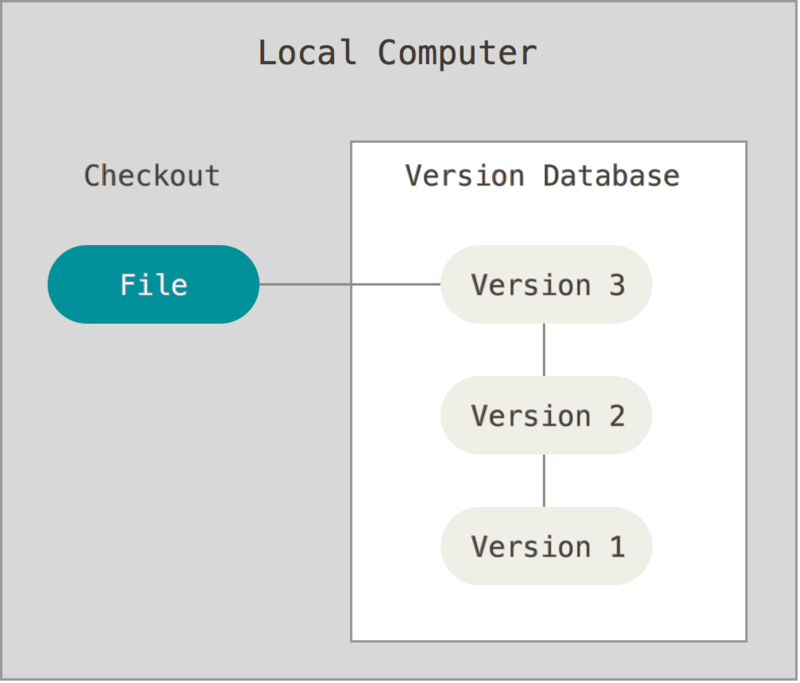
\includegraphics[width=0.5\textwidth]{vcs_local}
  
  \begin{itemize}
  \item Keeps differences between revisions in a local database
    \begin{itemize}
    \item Neat idea, as it saves disk space!
    \end{itemize}
  \item Can recreate what any file looked like at any point in time 
  \end{itemize}
\end{frame}


\begin{frame}
  \frametitle{Centralized Version Control systems}
  \framesubtitle{e.g., CVS, Subversion}
  \centering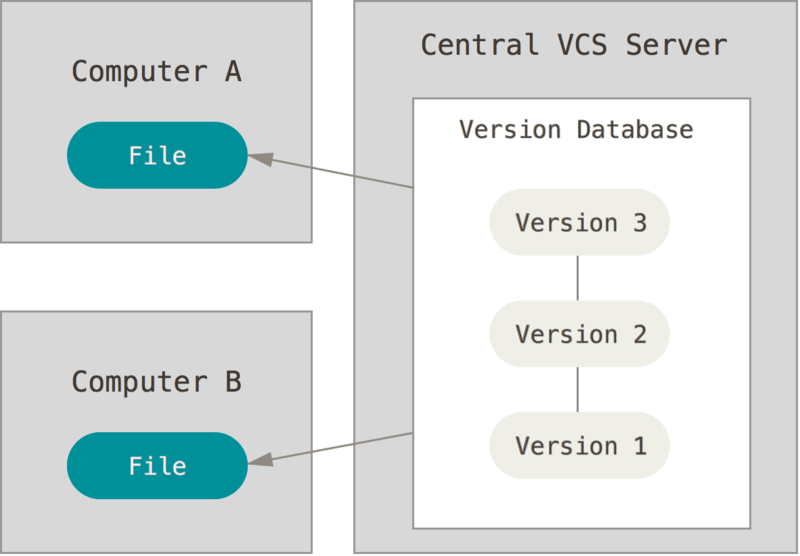
\includegraphics[width=0.5\textwidth]{vcs_centralized}
  
  \begin{itemize}
  \item Single server containing all the versioned files
    \begin{itemize}
    \item Clients can check out the files from the repository
    \end{itemize}
  \item Basic work-flow
    \begin{itemize}
    \item Check out a local working copy from the remote server
    \item Modify the working copy
    \item Commit the changes back to the repository
    \end{itemize}
  \item Most popular model through most of the '90
  \end{itemize}
\end{frame}


\begin{frame}
  \frametitle{Distributed version control system}
  \framesubtitle{e.g., git, mercurial}
  \centering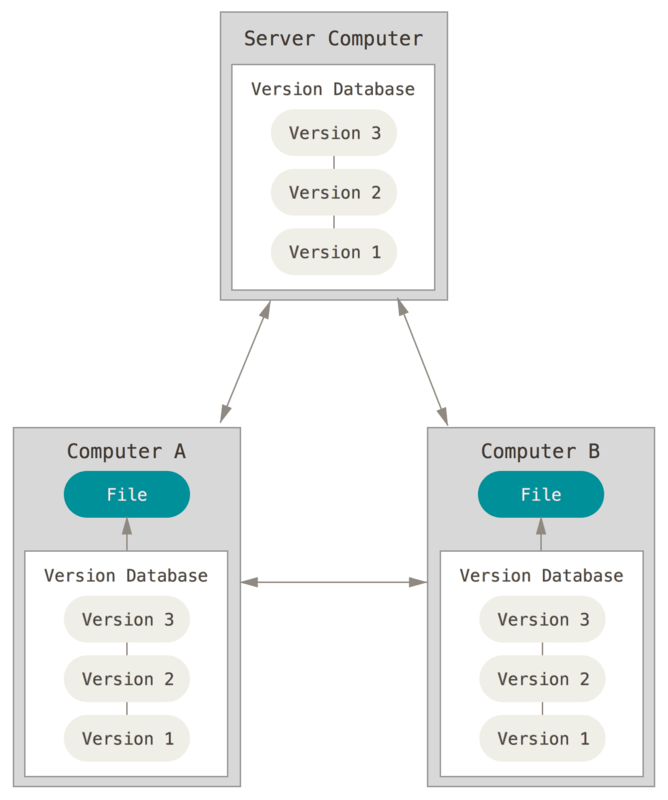
\includegraphics[width=0.5\textwidth]{vcs_distributed}
  
  \begin{itemize}
  \item Clients fully mirror the repository, including its full history
  \item Allows for a much richer variety of work-flows
  \end{itemize}
\end{frame}


\begin{frame}
  \frametitle{Versioning single files vs. the entire repository}
  \begin{itemize}
  \item Old VCS only tracked modification on a file-by-file basis
    \begin{itemize}
    \item i.e., CVS assigns revision numbers to the single files
    \end{itemize}
  \item All modern VCS track a whole commit as a new revision
    \begin{itemize}
    \item i.e., revisions are assigned to the repository
    \end{itemize}
  \item \alert{It makes a lot of sense to version the entire repository}
    \begin{itemize}
    \item Versioning single files can give a cozy feeling\ldots
    \item \ldots but when files interact with each other you need to know the
      status of the entire repository to reliably predict the output
    \end{itemize}
  \item \alert{Don't try and do the work that the VCS is supposed to do}
    \begin{itemize}
    \item Do not keep around multiple copies of the same file with
      a different suffix---the VCS is keeping track of the changes
    \item Do not copy and paste a block of code, comment the original and
      edit the second---this will make diffs harder to understand
    \end{itemize}
  \end{itemize}
\end{frame}



\begin{frame}
  \frametitle{Centralized vs. distributed VCS}
  \centering%
  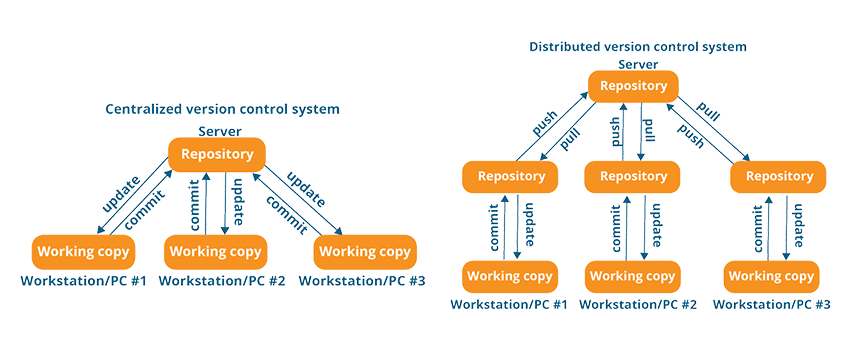
\includegraphics[width=0.9\textwidth]{vcs_centralized_vs_distributed}

  \begin{itemize}
  \item The centralized VCS work-flow is \emph{linear}
    \begin{itemize}
    \item Subversion assigns a progressive number to the repo at each commit
    \end{itemize}
  \item In a distributed system the work-flow is inherently \emph{non-linear}
    \begin{itemize}
    \item Any one given local repository is not ahead or behind any other
      repository---just different 
    \end{itemize}
  \item But then how do we assign revision in a distributed VCS?
  \end{itemize}
\end{frame}


\begin{frame}
  \frametitle{Digression: hash functions}
  \centering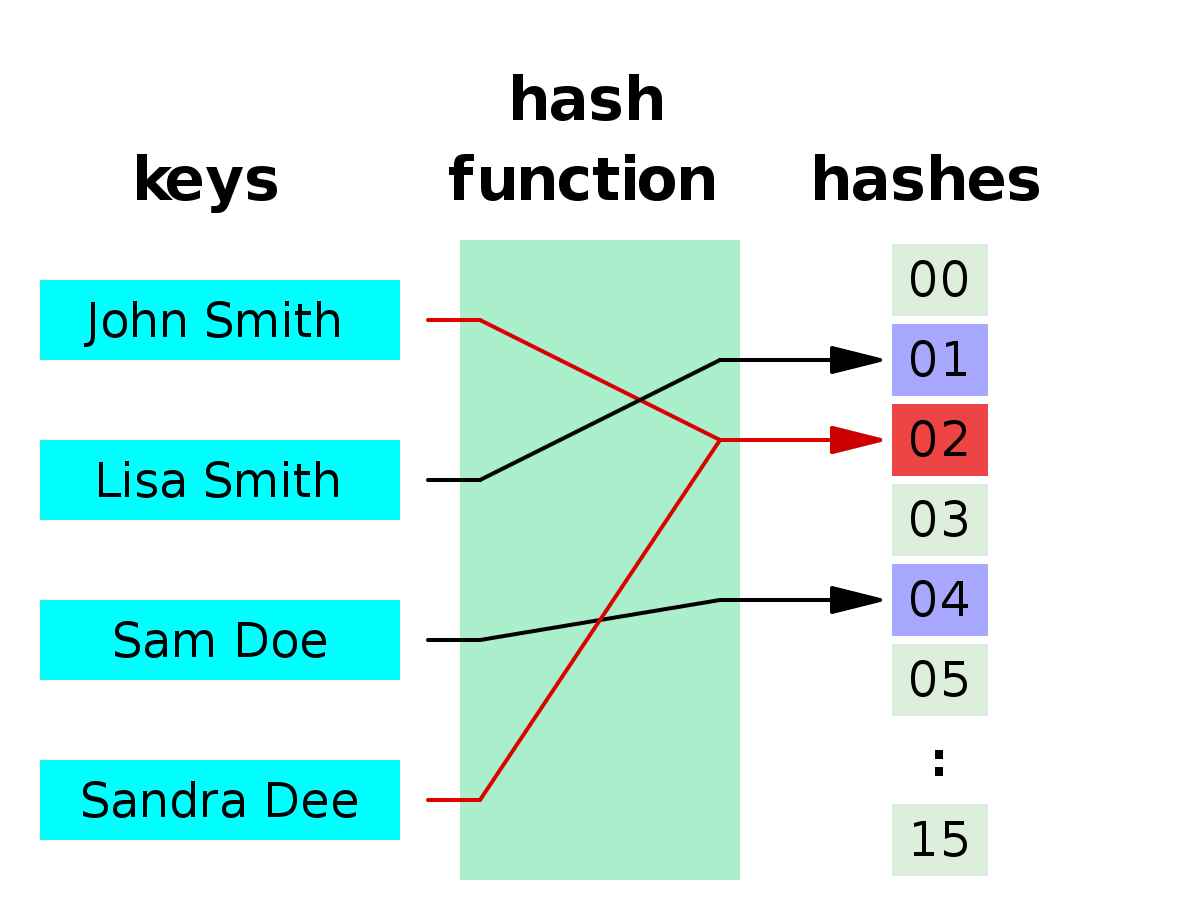
\includegraphics[width=0.5\textwidth]{hash}
  \begin{itemize}
  \item Ever heard of checksums? Or short versions of doodle links?
  \item \alert{A hash function maps data of arbitrary size to fixed-size values}
    \begin{itemize}
    \item e.g., anything to an integer
    \end{itemize}
  \item Good properties for a hash function
    \begin{itemize}
    \item Deterministic
    \item Uniform in the image space (minimize collisions)
    \item Fast to calculate (and, possibly, hard to invert)
    \end{itemize}
  \end{itemize}
\end{frame}


\begin{frame}[fragile]
  \frametitle{Hashing in Python}
  \begin{Verbatim}[label=\makebox{\url{https://github.com/lucabaldini/cmepda/tree/master/slides/latex/snippets/hashing.py}},commandchars=\\\{\}]
\PY{k}{print}\PY{p}{(}\PY{n+nb}{hash}\PY{p}{(}\PY{l+m+mi}{3}\PY{p}{)}\PY{p}{)}
\PY{k}{print}\PY{p}{(}\PY{n+nb}{hash}\PY{p}{(}\PY{l+m+mf}{3.}\PY{p}{)}\PY{p}{)}
\PY{k}{print}\PY{p}{(}\PY{n+nb}{hash}\PY{p}{(}\PY{l+m+mf}{3.001}\PY{p}{)}\PY{p}{)}
\PY{k}{print}\PY{p}{(}\PY{n+nb}{hash}\PY{p}{(}\PY{l+s+s1}{\PYZsq{}}\PY{l+s+s1}{hello}\PY{l+s+s1}{\PYZsq{}}\PY{p}{)}\PY{p}{)}
\PY{k}{print}\PY{p}{(}\PY{n+nb}{hash}\PY{p}{(}\PY{l+s+s1}{\PYZsq{}}\PY{l+s+s1}{Hello}\PY{l+s+s1}{\PYZsq{}}\PY{p}{)}\PY{p}{)}

[Output]
3
3
2305843009213443
-8080512805622017032
-8706679013462221575
\end{Verbatim}
  \begin{itemize}
  \item Every \emph{immutable} object is hashable in Python
    \begin{itemize}
    \item Each type gets its own algorithm
    \end{itemize}
  \item And why I am even bringing this up?
    \begin{itemize}
    \item Because in distributed VCS each commit gets its own has
    \end{itemize}
  \end{itemize}
  \begin{Verbatim}
[lbaldini@nbbaldini slides]$ git rev-parse HEAD
e0a170d789865179d99506c9f067f3875292524b
  \end{Verbatim}
\end{frame}


\begin{frame}
  \frametitle{More terminology}
  \centering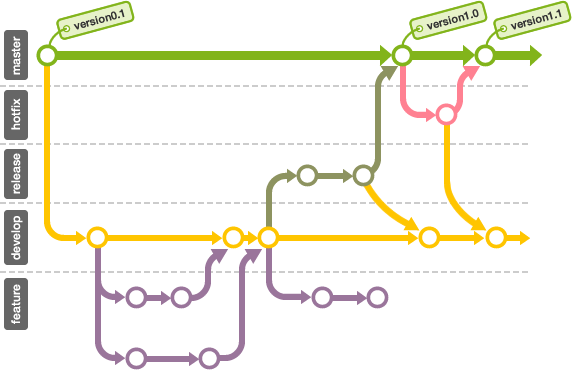
\includegraphics[width=0.6\textwidth]{vcs_workflow}
  
  \begin{itemize}
  \item \alert{Branches}: alternative paths where more copies of the same files
    develop in different ways independently
  \item \alert{Master, or trunk, or tip}: the unique line of development that
    is not a branch
  \item \alert{Merge}: application of two sets of changes to a set of files
  \item \alert{Conflict}: changes to the same file by two or more developers
    that the system is unable to reconcile
  \end{itemize}
\end{frame}


\begin{frame}[fragile]
  \frametitle{Basic git commands}
  \framesubtitle{Try \texttt{git -{}-help}}
  \begin{Verbatim}
start a working area (see also: git help tutorial)
   clone      Clone a repository into a new directory

work on the current change (see also: git help everyday)
   add        Add file contents to the index
   mv         Move or rename a file, a directory, or a symlink
   rm         Remove files from the working tree and from the index

examine the history and state (see also: git help revisions)
   log        Show commit logs
   show       Show various types of objects
   status     Show the working tree status

grow, mark and tweak your common history
   branch     List, create, or delete branches
   checkout   Switch branches or restore working tree files
   commit     Record changes to the repository
   diff       Show changes between commits, commit and working tree, etc
   merge      Join two or more development histories together
   tag        Create, list, delete or verify a tag object signed with GPG

collaborate (see also: git help workflows)
   pull       Fetch from and integrate with another repository or a local branch
   push       Update remote refs along with associated objects
  \end{Verbatim}
\end{frame}


\begin{frame}[fragile]
  \frametitle{A simple but realistic work-flow}
  \begin{enumerate}
  \item Clone your repository
  \item Create a new branch and check it out
  \item Do all you have to do
  \item Add the new files, commit your modified files
  \item Create a pull request
  \item Have your pull request reviewed
  \item Merge the branch on the master
  \item Tag the master
  \end{enumerate}
\end{frame}


\begin{frame}[fragile]
  \frametitle{A few suggestions}
  \begin{itemize}
  \item Pick a sensible name for your branches
    \begin{itemize}
    \item Try and express your \emph{intent}
    \item Examples of bad names: \verb|my_branch|, \verb|new_branch|,
      \verb|awesome_branch|
    \item Examples of reasonable names: \verb|update_data_format|,
      \verb|fix_issue_2376|
    \end{itemize}
  \item Try and isolate related changes in the smallest possible subset
    \begin{itemize}
    \item Attack one problem at a time
    \item Do not mix unrelated issues in the same pull request
    \item The smallest the pull request, the easiest the review
    \end{itemize}
  \item Do not try and do what the VCS is suppose to take care of
    \begin{itemize}
    \item Do not commit to the repository multiple versions of the same
      file---the VCS is perfectly capable of tracking the changes
    \item Do not copy and paste chunck of code, comment the old version and
      tweak the new---this will make diffs harder to read
    \end{itemize}
  \item VCS are good at handling text files
    \begin{itemize}
    \item Do not commit large binary files (e.g., data sets) to your
      repository---it will stay there forever
    \end{itemize}
  \end{itemize}
\end{frame}

\begin{frame}
  \frametitle{Logistical remarks}
  \begin{itemize}
  \item Which VCS should I use?
    \begin{itemize}
    \item Everybody else is using git, these days---you might as well stick
      to that
    \end{itemize}
  \item Hosting: shall I set up a server myself or use a hosting service?
    \begin{itemize}
    \item This is a no brainer: use a service (e.g., github, gitlab, bitbucket)
    \end{itemize}
  \item What shall I use version control for?
    \begin{itemize}
    \item Your thesis
    \item Your papers (or lab assignments)
    \item Your webpage (if you have one)
    \item The invitations for your wedding
    \item Really: everything you care about!
    \end{itemize}
  \item Shall I care about the license?
    \begin{itemize}
    \item Definitely: make easy for others to use and adapt your code
      (unless you have good reasons not to)
    \item GNU General Public License v3.0 is a good choice for code
    \item Creative Commons Attribution-ShareAlike 4.0 is a good choice for
      documents
    \end{itemize}
  \end{itemize}
\end{frame}


\begin{frame}
  \frametitle{References}
  \scriptsize
  \begin{itemize}
  \item \url{https://en.wikipedia.org/wiki/Version_control}
  \item \url{https://git-scm.com/book/en/v2/Getting-Started-About-Version-Control}
  \item \url{https://en.wikipedia.org/wiki/Hash_function}
  \item \url{https://git-scm.com/}
  \item \url{https://github.com/}
  \item \url{https://bitbucket.org/}
  \item \url{https://about.gitlab.com/}
  \end{itemize}
\end{frame}



\end{document}
